
%% bare_conf.tex
%% V1.3
%% 2007/01/11
%% by Michael Shell
%% See:
%% http://www.michaelshell.org/
%% for current contact information.
%%
%% This is a skeleton file demonstrating the use of IEEEtran.cls
%% (requires IEEEtran.cls version 1.7 or later) with an IEEE conference paper.
%%
%% Support sites:
%% http://www.michaelshell.org/tex/ieeetran/
%% http://www.ctan.org/tex-archive/macros/latex/contrib/IEEEtran/
%% and
%% http://www.ieee.org/

%%*************************************************************************
%% Legal Notice:
%% This code is offered as-is without any warranty either expressed or
%% implied; without even the implied warranty of MERCHANTABILITY or
%% FITNESS FOR A PARTICULAR PURPOSE! 
%% User assumes all risk.
%% In no event shall IEEE or any contributor to this code be liable for
%% any damages or losses, including, but not limited to, incidental,
%% consequential, or any other damages, resulting from the use or misuse
%% of any information contained here.
%%
%% All comments are the opinions of their respective authors and are not
%% necessarily endorsed by the IEEE.
%%
%% This work is distributed under the LaTeX Project Public License (LPPL)
%% ( http://www.latex-project.org/ ) version 1.3, and may be freely used,
%% distributed and modified. A copy of the LPPL, version 1.3, is included
%% in the base LaTeX documentation of all distributions of LaTeX released
%% 2003/12/01 or later.
%% Retain all contribution notices and credits.
%% ** Modified files should be clearly indicated as such, including  **
%% ** renaming them and changing author support contact information. **
%%
%% File list of work: IEEEtran.cls, IEEEtran_HOWTO.pdf, bare_adv.tex,
%%                    bare_conf.tex, bare_jrnl.tex, bare_jrnl_compsoc.tex
%%*************************************************************************

\documentclass[journal,onecolumn]{IEEEtran}
\usepackage{blindtext, graphicx, listings, xcolor, float}
\usepackage[spanish]{babel}
\usepackage[utf8]{inputenc}

\definecolor{commentgreen}{RGB}{2,112,10}
\definecolor{eminence}{RGB}{108,48,130}
\definecolor{weborange}{RGB}{255,165,0}
\definecolor{frenchplum}{RGB}{129,20,83}

\lstset {
 	language=C++,
    frame=tb,
    tabsize=4,
    showstringspaces=false,
    numbers=left,
    %upquote=true,
    commentstyle=\color{commentgreen},
    keywordstyle=\color{eminence},
    stringstyle=\color{red},
    basicstyle=\small\ttfamily, % basic font setting
    emph={git,mvn,export,hadoop,pig,hive,oozie,LOAD,REGISTER,USING,AS,FILTER,BY,AND,
    GROUP,FOREACH,GENERATE,MAX,STORE,INTO,INSERT,OVERWRITE,DYRECTORY,SELECT,FROM,WHERE,IN,ADD},
    emphstyle={\color{blue}},
    escapechar=\&,
    % keyword highlighting
    classoffset=1, % starting new class
    otherkeywords={>,<,;,!,=,~},
    morekeywords={>,<,;,!,=,~},
    keywordstyle=\color{weborange},
    classoffset=0,
    extendedchars=true,
    literate={á}{{\'a}}1 {ã}{{\~a}}1 {é}{{\'e}}1 {í}{{\'i}}1 {ó}{{\'o}}1 {ú}{{\'u}}1
}

% correct bad hyphenation here
%\hyphenation{op-tical net-works semi-conduc-tor}


\begin{document}
%
% paper title
% can use linebreaks \\ within to get better formatting as desired
\title{MapReduce, Pig, HCatalog and Oozie:\\ Una guía práctica}


% author names and affiliations
% use a multiple column layout for up to three different
% affiliations
\author{\IEEEauthorblockN{Luis F. Rivera}
\IEEEauthorblockA{\\Departamento Académico de Tecnologías de Información y Comunicaciones (TICs)\\
Universidad Icesi\\
Cali, Colombia\\
Email: lfrivera@icesi.edu.co}
}

% conference papers do not typically use \thanks and this command
% is locked out in conference mode. If really needed, such as for
% the acknowledgment of grants, issue a \IEEEoverridecommandlockouts
% after \documentclass

% for over three affiliations, or if they all won't fit within the width
% of the page, use this alternative format:
% 
%\author{\IEEEauthorblockN{Michael Shell\IEEEauthorrefmark{1},
%Homer Simpson\IEEEauthorrefmark{2},
%James Kirk\IEEEauthorrefmark{3}, 
%Montgomery Scott\IEEEauthorrefmark{3} and
%Eldon Tyrell\IEEEauthorrefmark{4}}
%\IEEEauthorblockA{\IEEEauthorrefmark{1}School of Electrical and Computer Engineering\\
%Georgia Institute of Technology,
%Atlanta, Georgia 30332--0250\\ Email: see http://www.michaelshell.org/contact.html}
%\IEEEauthorblockA{\IEEEauthorrefmark{2}Twentieth Century Fox, Springfield, USA\\
%Email: homer@thesimpsons.com}
%\IEEEauthorblockA{\IEEEauthorrefmark{3}Starfleet Academy, San Francisco, California 96678-2391\\
%Telephone: (800) 555--1212, Fax: (888) 555--1212}
%\IEEEauthorblockA{\IEEEauthorrefmark{4}Tyrell Inc., 123 Replicant Street, Los Angeles, California 90210--4321}}




% use for special paper notices
%\IEEEspecialpapernotice{(Invited Paper)}




% make the title area
\maketitle


\begin{abstract}
My abstract.
\end{abstract}
% IEEEtran.cls defaults to using nonbold math in the Abstract.
% This preserves the distinction between vectors and scalars. However,
% if the journal you are submitting to favors bold math in the abstract,
% then you can use LaTeX's standard command \boldmath at the very start
% of the abstract to achieve this. Many IEEE journals frown on math
% in the abstract anyway.

% Note that keywords are not normally used for peerreview papers.
\begin{IEEEkeywords}
map reduce, pig, hive, hcatalog, oozie.
\end{IEEEkeywords}






% For peer review papers, you can put extra information on the cover
% page as needed:
% \ifCLASSOPTIONpeerreview
% \begin{center} \bfseries EDICS Category: 3-BBND \end{center}
% \fi
%
% For peerreview papers, this IEEEtran command inserts a page break and
% creates the second title. It will be ignored for other modes.
\IEEEpeerreviewmaketitle



\section{Introduction}
\textit{Apache Hadoop} es un \textit{framework} de código abierto para el almacenamiento y procesamiento de grandes volúmenes de datos \footnote{https://hortonworks.com/apache/hadoop/}. Generalmente, Hadoop es considerado como un ecosistema, en el que habitan, entre otras, herramientas como \textit{Apache Hive}, \textit{Apache Pig}, y \textit{Apache Oozie}, las cuales fueron concebidas con el objetivo de complementar los cuatro elementos principales del core de Hadoop (HDFS, MapReduce, YARN, y Common)\footnote{http://www.bmc.com/guides/hadoop-ecosystem.html}. \\

El objetivo principal de este proyecto consiste en analizar un subconjunto de las herramientas pertenecientes al ecosistema de Hadoop, desde la perspectiva de la infraestructura computacional necesaria ponerlas en marcha y de los principales atributos de calidad involucrados en el uso de las mismas. Para este propósito, un escenario de pruebas controlado fue configurado usando la versión 5.10.1 de \textit{Cloudera Manager} (CDH 5.10.1). Dicha configuración fue establecida como se muestra en la figura \ref{deployment_diagram}

\begin{figure}[H]
\label{deployment_diagram}
  \centering
      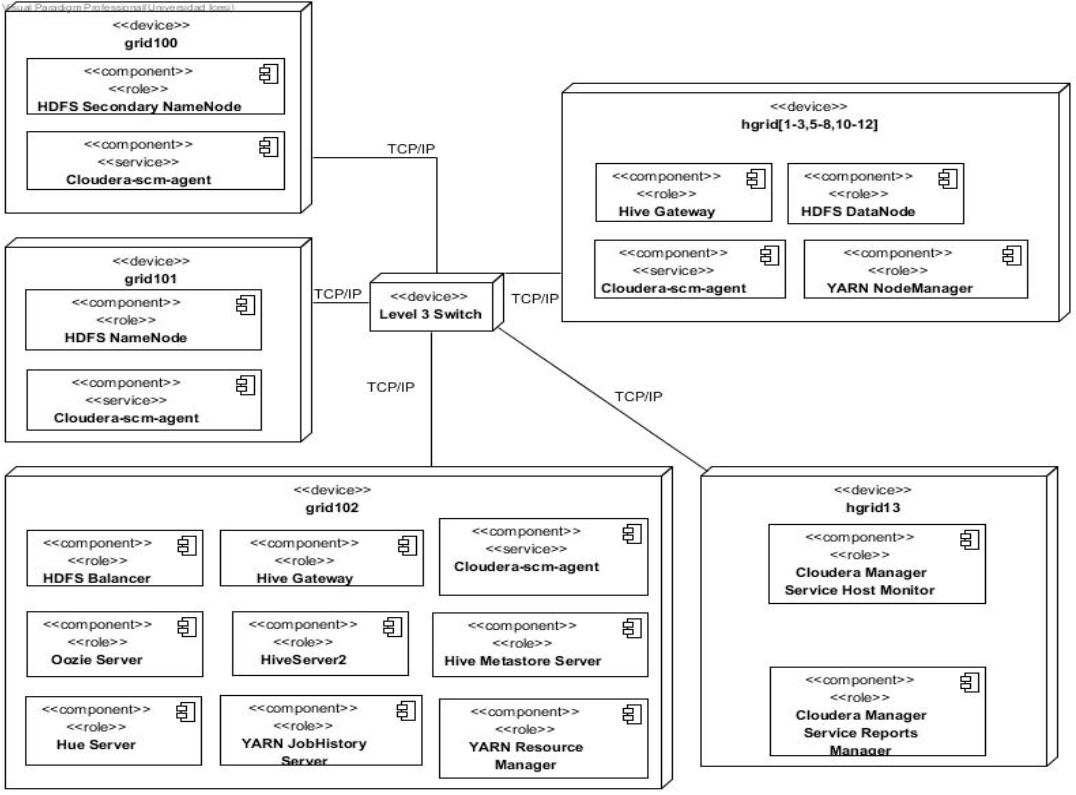
\includegraphics[width=\textwidth, height=2.5in]{fig/deployment}
  \caption{Diagrama de despliegue de la configuración de CDH 5.10.1 en el laboratorio \textit{LIASON} de la Universidad Icesi.}
\end{figure}

Cada uno de los casos de estudio de minería de datos presente en este proyecto se basa en los datos provistos por el \textit{National Climatic Data Center} (NCDC). Dichos datos son recolectados por medio de sensores climáticos, los cuales recolectan información cada hora, de forma diaria, en distintas estaciones a lo largo del mundo. Dichos datos se encuentran registrados a través de lineas en archivos de texto. La figura \ref{dataset} muestra la descripción del conjunto de datos mencionado previamente. \\

\begin{figure}[H]
\label{dataset}
  \centering
      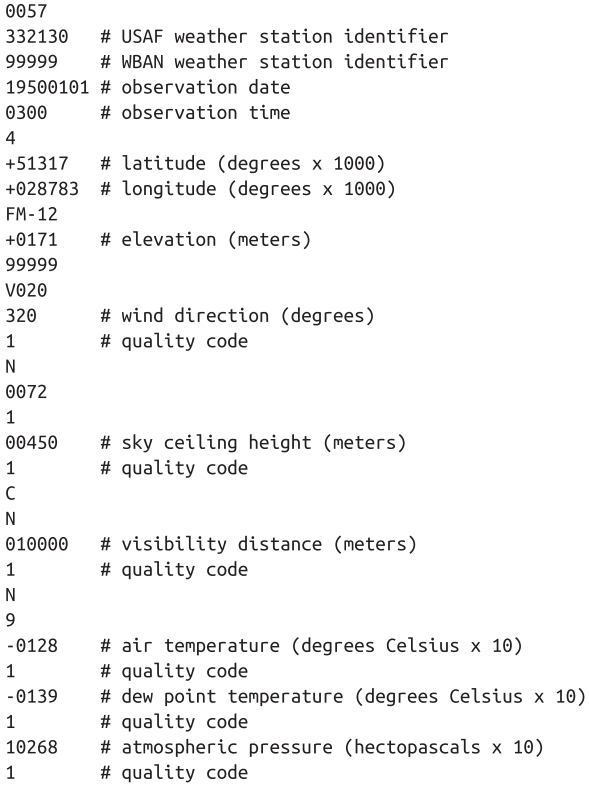
\includegraphics[width=\textwidth, height=3.5in]{fig/dataset}
  \caption{Descripción del conjunto de datos. Tomado de \cite{White:2012:HDG:2285539}}
\end{figure}

El resto del presente documento se encuentra distribuido como se muestra a continuación. En la sección 1 se describen formalmente el objetivo general y los objetivos objetivos específicos del proyecto. En la sección 2 se presentan los tipos de pruebas ejecutadas sobre las herramientas \textit{MapReduce}, \textit{Apache Pig}, y \textit{Apache Hive} para entender la diferencia entre los tiempos de ejecución de las mismas. En la sección 3 se ilustran las distintas pruebas llevadas a cabo sobre las herramientas \textit{Apache Pig} y \textit{HCatalog} para verificar la posibilidad de extender las funcionalidades y capacidades provistas por \textit{Pig}. En la sección 4 se detallan las pruebas realizadas sobre \textit{Apache Ooozie}, las cuales buscan evidenciar la re-usabilidad y mantenibilidad de las aplicaciones desarrolladas sobre esta herramienta. La sección 5 muestra los resultados de la ejecución de las pruebas descritas previamente. En la sección 6 se presentan las conclusiones del presente trabajo. Finalmente, la sección 7 muestra las posibilidades de trabajo futuro que se podrían desarrollar a partir de lo que aquí se presenta.

\section{Objetivos del proyecto}
El objetivo general del proyecto consiste en analizar, desde un punto de vista arquitectónico, algunas de las herramientas que conforman el ecosistema de Hadoop. Para esto, se estudiará MapReduce, Apache Pig, Apache Hive, HCatalog, y Apache Oozie desde la perspectiva de los atributos de calidad de desempeño (\textit{performance}), reusabilidad (\textit{reusability}), extensibilidad (\textit{extensibility}), y mantenibilidad (\textit{maintainability})). A continación se describen los objetivos específicos del proyecto y los atributos de calidad asociados a cada uno de estos. \\

\begin{enumerate}

\item
{
Construir y ejecutar un caso de estudio bajo un entorno de pruebas controlado, el cual permita, en una primera instancia, entender la diferencia en los tiempos de ejecución de MapReduce, ApachePig, y Apache Hive. Atributo de calidad relacionado: \textit{performance}.
}

\item
{
Construir y ejecutar un caso de estudio bajo un entorno de pruebas controlado, el cual permita, en una primera instancia, entender si Apache Pig podría aprovechar las ventajas de Apache Hive a través de HCatalog. Atributos de calidad relacionados: \textit{performance, extensibility}.
}

\item
{
Construir y ejecutar un caso de estudio bajo un entorno de pruebas controlado, el cual permita, en una primera instancia, entender la posibilidad de re-uso y la facilidad de mantener \textit{workflows} en Apache Oozie. Atributos de calidad relacionados: \textit{reusability, maintainability}.
}

\end{enumerate}


\section{MapReduce, Pig y Hive}
En esta sección se presentan las ejecuciones realizadas con MapReduce, Apache Pig, y Apache Hive para el cálculo de la temperatura máxima registrada por año para el objetivo específico 1 del presente proyecto.

\subsection{Problema tratado}

Determinar la temperatura máxima registrada por año para los datos consignados en el dataset del NCDC.


\subsection{Ejecución con MapReduce}

A continuación se detallan los pasos necesarios para ejecutar el programa \textit{MaxTemperature} en su versión MapReduce-Java. \\

\subsubsection{Preparación}

Inicialmente, es necesario compilar el código fuente del programa \textit{MaxTemperature} en su versión Java. Para hacer esto, es necesario clonar el repositorio del libro \textit{Hadoop: The Definitive Guide}\footnote{Repositorio provisto por Tom White en https://github.com/tomwhite/hadoop-book}. Una vez hecho lo anterior, se debe proceder a compilar los archivos fuente necesarios mediante \textit{Maven}.Finalmente, la ruta del archivo .jar compilado deberá establecerse en una variable de entorno llamada \textit{HADOOP\_CLASSPATH}. 

\begin{lstlisting}[linewidth=\columnwidth,breaklines=true]
//Clonación del repositorio.
git clone &https://github.com/tomwhite/hadoop-book.git&

// Compilación del código fuente.
mvn package &-&DskipTests

// Definición del classpath de Hadoop.
export HADOOP_CLASSPATH&=&/home/sas6/Oozie&-&Pig&-&HCatalog&-&Demos/assets/&hadoop-&examples&.&jar
\end{lstlisting}


\subsubsection{Ejecución del programa MaxTemperature}

Una vez compilado el código fuente y definida la variable de entorno correspondiente, se procede a ejecutar el programa \textit{MaxTemperature}.

\begin{lstlisting}[linewidth=\columnwidth,breaklines=true]
hadoop MaxTemperature /user/&hive&/warehouse/weather_external/full_data&.&txt out_mr_300GB
\end{lstlisting}


\subsubsection{Seguimiento a la ejecución del programa}

Una vez iniciada la ejecución del programa, es posible monitorear el progreso del mismo por medio de la consola donde éste se ejecutó o por medio de la interfaz gráfica de YARN.

\begin{figure}[H]
  \centering
      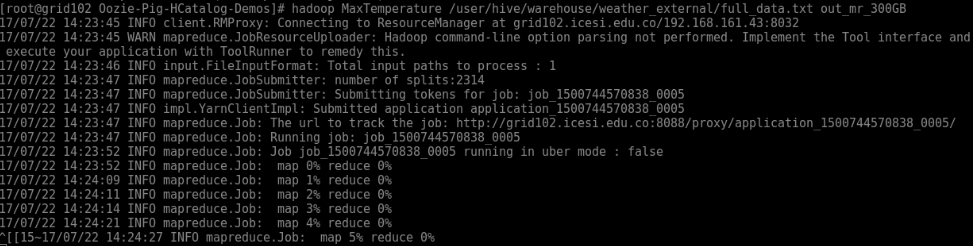
\includegraphics[width=\textwidth, height=1.5in]{fig/04/00}
  \caption{Monitoreo de la ejecución del programa \textit{MaxTemperature} en MapReduce por medio de la consola en donde éste se ejecutó.}
\end{figure}

\begin{figure}[H]
  \centering
      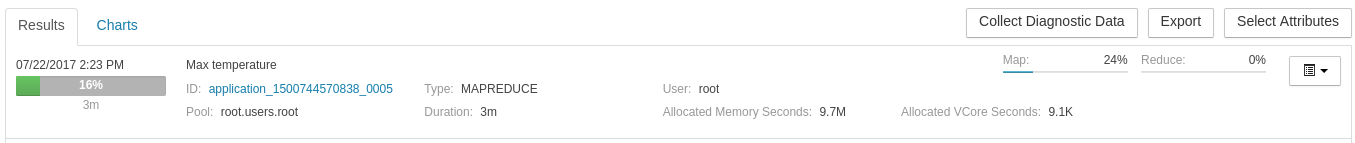
\includegraphics[width=\textwidth, height=1.0in]{fig/04/01}
  \caption{Monitoreo de la ejecución del programa \textit{MaxTemperature} en MapReduce por medio de la interfaz de YARN.}
\end{figure}

\begin{figure}[H]
  \centering
      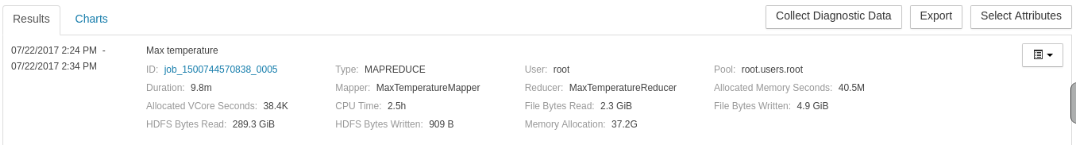
\includegraphics[width=\textwidth, height=1.0in]{fig/04/02}
  \caption{Ejecución finalizada.}
\end{figure}

\subsection{Ejecución con Hive}

A continuación se detallan los pasos necesarios para ejecutar el programa \textit{MaxTemperature} en su versión Apache Hive. \\

\subsubsection{Ejecución con la consola de Hive}

El siguiente script detalla la ejecución del programa \textit{MaxTemperature} en su versión Apache Hive.

\begin{lstlisting}[linewidth=\columnwidth,breaklines=true]
ADD jar /usr/lib/&hive&/lib/&hive&-contrib-1.1.0-cdh5.10.1.jar; 
INSERT OVERWRITE DIRECTORY 'out_max_hive_300GB' 
SELECT observation_date_year, MAX(air_temperature) 
FROM weather_managed 
WHERE air_temperature != 9999 AND at_quality_code IN (0,1,4,5,9) 
GROUP BY observation_date_year;
\end{lstlisting} 

\subsubsection{Seguimiento a la ejecución del programa}

El monitoreo de la ejecución del programa podrá realizarse a través de la interfaz gráfica de YARN, o por la información proporcionada por el Job History Server.

\begin{figure}[H]
  \centering
      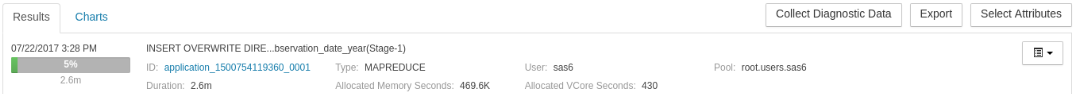
\includegraphics[width=\textwidth, height=0.6in]{fig/04/06}
  \caption{Monitoreo de la ejecución del programa \textit{MaxTemperature} en Hive por medio de la interfaz de YARN. }
\end{figure}

\begin{figure}[H]
  \centering
      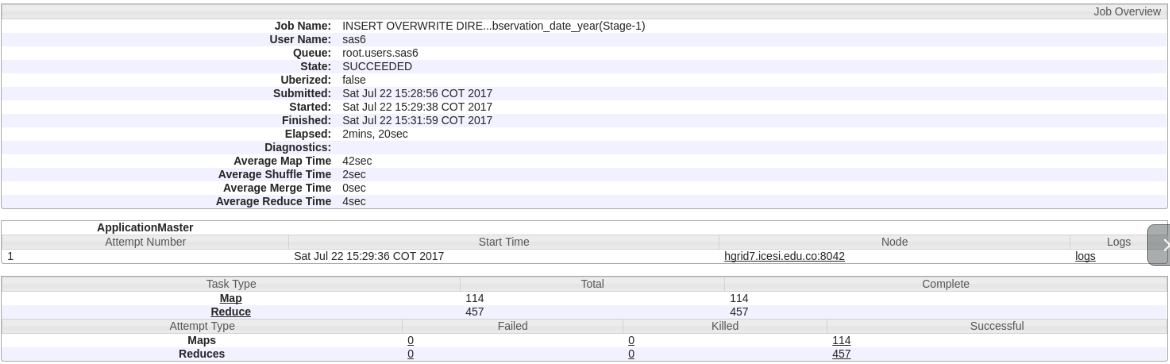
\includegraphics[width=\textwidth, height=2.5in]{fig/04/07}
  \caption{Ejecución finalizada, vista desde el Job History Server.}
\end{figure}


\subsection{Ejecución con Pig}

A continuación se detallan los pasos necesarios para ejecutar el programa \textit{MaxTemperature} en su versión Apache Pig. \\

\subsubsection{Definición del script en PigLatin}

El siguiente script contiene el código utilizado utilizado para ejecutar el programa \textit{MaxTemperature} en su versión PigLatin. En las dos primeras lineas del script se detalla el uso de una UDF (\textit{User defined function}), provista por Tom White, para la lectura de registros a partir de la definición de rangos de lectura para sus atributos. El contenido del script fue guardado en un archivo llamado \textit{max-temp.pig}.

\begin{lstlisting}[linewidth=\columnwidth,breaklines=true]
REGISTER $load_loc;
records = LOAD '$in_s1' USING &com.hadoopbook.pig.CutLoadFunc&('16-19,88-92,93-93') AS (year:int, temperature:int, quality:int); 
filtered_records = FILTER records BY temperature != 9999 AND &com.hadoopbook.pig.IsGoodQuality&(quality);
grouped_records = GROUP filtered_records BY year;
max_temp = FOREACH grouped_records GENERATE group,MAX(filtered_records.temperature);
STORE max_temp INTO '$out_max';   
\end{lstlisting} 


\subsubsection{Definición de los parámetros del script}

Una vez definido el script en PigLatin, se procede a definir en un nuevo archivo los parámetros necesarios para la correcta ejecución del script. Los parámetros mencionados fueron guardados en un archivo llamado \textit{max.param}.

\begin{lstlisting}[linewidth=\columnwidth,breaklines=true]
# Load function location.
load_loc=/home/sas6/Oozie-Pig-HCatalog-Demos/assets/&pig&-examples.jar
# Input.
in_s1=/user/&hive&/warehouse/weather_external/full_data.txt
# Output.
out_max=out_max_pig
\end{lstlisting}

\subsubsection{Ejecución con Grunt en modo \textit{batch}}

A continuación se detalla el comando utilizado para ejecutar el programa \textit{MaxTemperature} mediante el modo \textit{batch} de Grunt.

\begin{lstlisting}[linewidth=\columnwidth,breaklines=true]
pig -param_file /home/sas6/Oozie-Pig-HCatalog-Demos/scripts/&pig&/300GB/max.param /home/sas6/Oozie-Pig-HCatalog-Demos/src/&pig&/max-temp.&pig&
\end{lstlisting}

\subsubsection{Seguimiento a la ejecución del programa}

El monitoreo de la ejecución del programa podrá realizarse a través de Grunt, por medio de la interfaz gráfica de YARN, o por la información proporcionada por el Job History Server.

\begin{figure}[H]
  \centering
      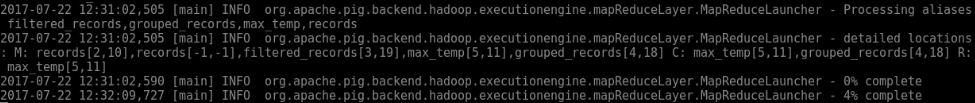
\includegraphics[width=\textwidth, height=1.0in]{fig/04/03}
  \caption{Monitoreo de la ejecución del programa \textit{MaxTemperature} en Pig por medio de la consola Grunt desde donde se ejecutó.}
\end{figure}

\begin{figure}[H]
  \centering
      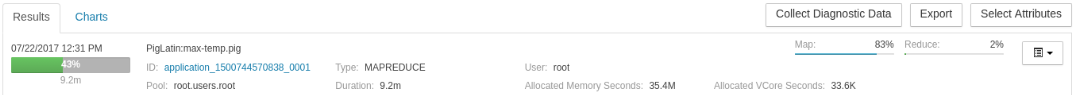
\includegraphics[width=\textwidth, height=0.6in]{fig/04/04}
  \caption{Monitoreo de la ejecución del programa \textit{MaxTemperature} en Pig por medio de la interfaz de YARN.}
\end{figure}

\begin{figure}[H]
  \centering
      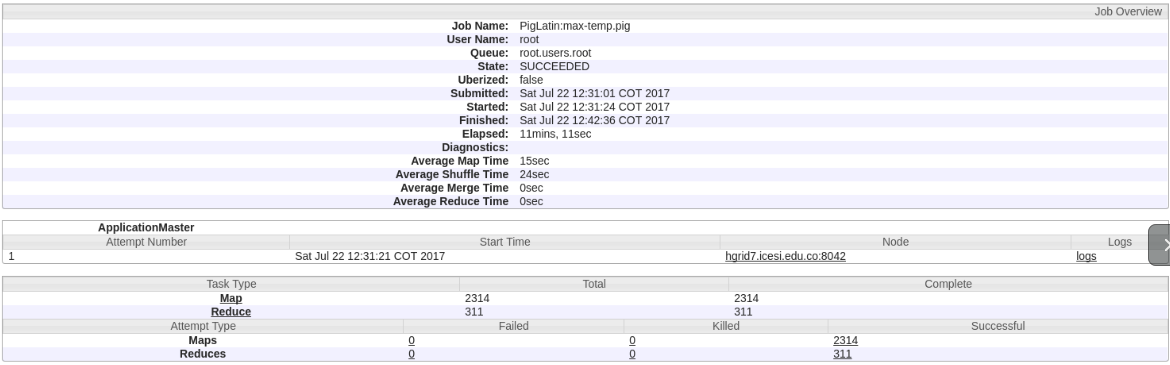
\includegraphics[width=\textwidth, height=2.5in]{fig/04/05}
  \caption{Ejecución finalizada, vista desde el Job History Server.}
\end{figure}

\section{Escalabilidad de Pig}

A continuación se detallan los pasos necesarios para ejecutar el programa \textit{AverageTemperatureCount} con Apache Pig para el objetivo específico 2 del presente proyecto \\

\subsection{Problema tratado}

Determinar la temperatura promedio registrada por año y el número de estaciones meteorológicas utilizadas para su cálculo, teniendo como base los datos consignados en el dataset del NCDC.

\subsection{Definición del script en PigLatin}

El siguiente script contiene el código utilizado utilizado para ejecutar el programa \textit{AverageTemperatureCount} en su versión PigLatin. En las dos primeras lineas del script se detalla el uso de una UDF (\textit{User defined function}), provista por Tom White, para la lectura de registros a partir de la definición de rangos de lectura para sus atributos. El contenido del script fue guardado en un archivo llamado \textit{avg-count-temp-scalability.pig}.

\begin{lstlisting}[linewidth=\columnwidth,breaklines=true]
REGISTER $load_loc; 
records = LOAD '$in_s1' USING com.hadoopbook.&pig&.CutLoadFunc('16-19,88-92,93-93') AS (year:int, temperature:int, quality:int);
filtered_records = FILTER records BY temperature != 9999 AND com.hadoopbook.&pig&.IsGoodQuality(quality); 
grouped_records = GROUP filtered_records BY year; 
mean_count_temp = FOREACH grouped_records GENERATE group,AVG(filtered_records.temperature),COUNT(filtered_records); 
STORE mean_count_temp INTO '$out_max'; 
\end{lstlisting} 


\subsection{Definición de los parámetros del script}

Una vez definido el script en PigLatin, se procede a definir en un nuevo archivo los parámetros necesarios para la correcta ejecución del script. Los parámetros mencionados fueron guardados en un archivo llamado \textit{avg-count-temp-scalability.param}.

\begin{lstlisting}[linewidth=\columnwidth,breaklines=true]
# Load function location.
load_loc=/home/sas6/Oozie-Pig-HCatalog-Demos/assets/&pig&-examples.jar
# Input.
in_s1=/user/&hive&/warehouse/weather_external/full_data.txt
# Output.
out_max=out_scalabity_pig
\end{lstlisting}

\subsection{Ejecución con Grunt en modo \textit{batch}}

A continuación se detalla el comando utilizado para ejecutar el programa \textit{AverageTemperatureCount} mediante el modo \textit{batch} de Grunt.

\begin{lstlisting}[linewidth=\columnwidth,breaklines=true]
pig -param_file /home/sas6/Oozie-Pig-HCatalog-Demos/scripts/&pig&/300GB/avg-count-scalabity.param /home/sas6/Oozie-Pig-HCatalog-Demos/src/&pig&/avg-count-temp-scalability.&pig&
\end{lstlisting}

\subsection{Seguimiento a la ejecución del programa}

El monitoreo de la ejecución del programa podrá realizarse a través de Grunt, por medio de la interfaz gráfica de YARN, o por la información proporcionada por el Job History Server.

\begin{figure}[H]
  \centering
      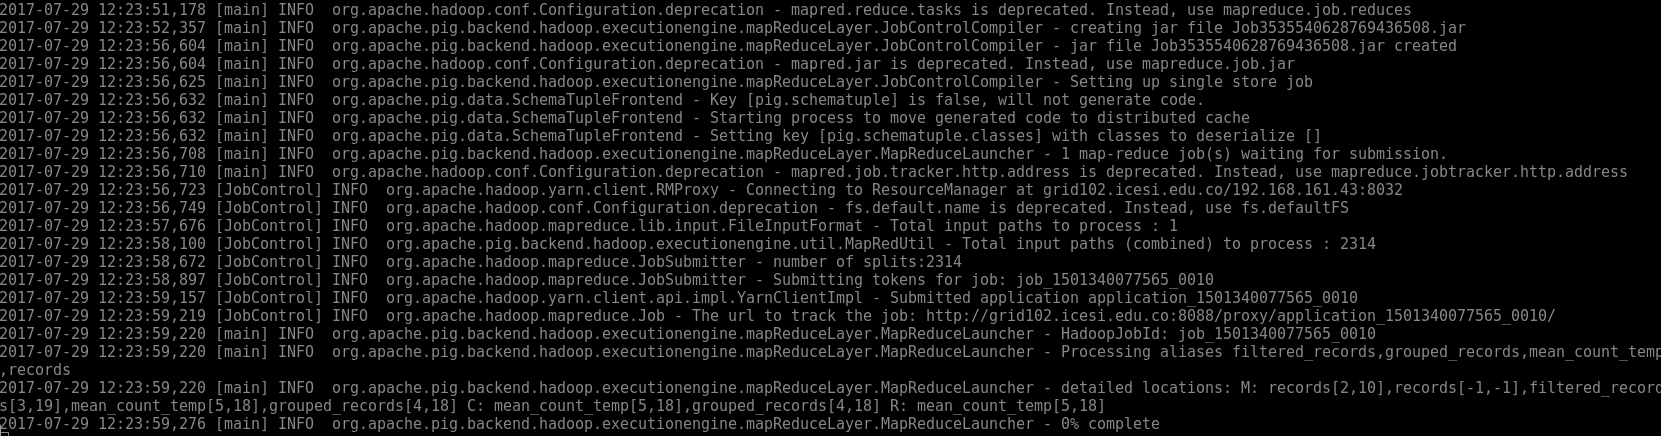
\includegraphics[width=\textwidth, height=2.0in]{fig/03/01}
  \caption{Monitoreo de la ejecución del programa \textit{AverageTemperatureCount} en Pig por medio de la consola Grunt desde donde se ejecutó.}
\end{figure}

\begin{figure}[H]
  \centering
      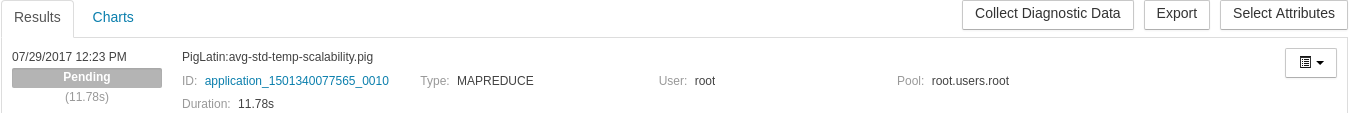
\includegraphics[width=\textwidth, height=0.8in]{fig/03/02}
  \caption{Monitoreo de la ejecución del programa \textit{AverageTemperatureCount} en Pig por medio de la interfaz de YARN.}
\end{figure}

\begin{figure}[H]
  \centering
      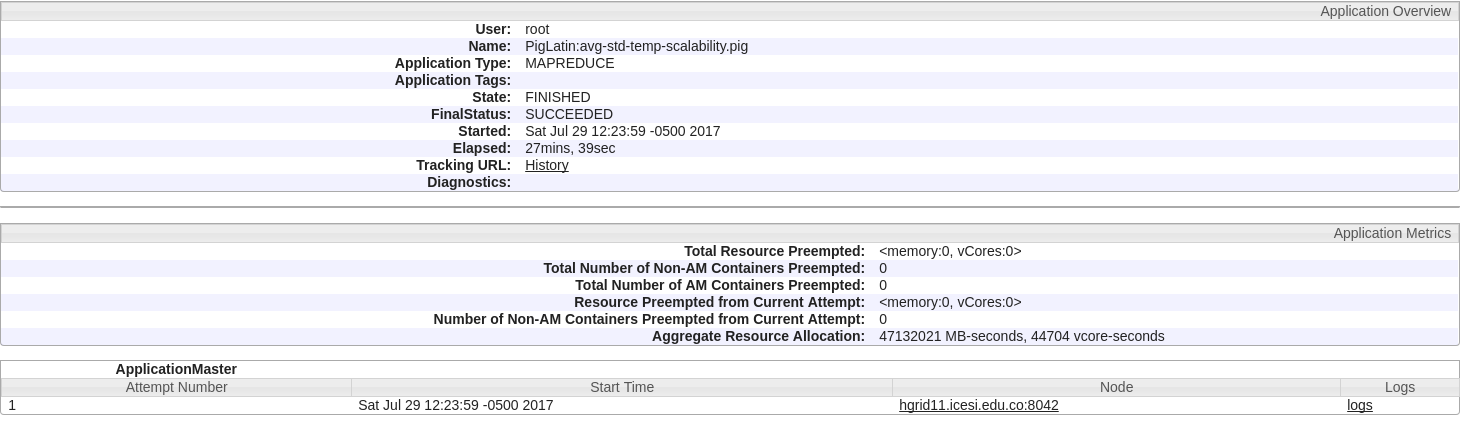
\includegraphics[width=\textwidth, height=2.7in]{fig/03/03}
  \caption{Ejecución finalizada, vista desde el Job History Server.}
\end{figure}

\section{Pig and HCatalog}
En esta sección se presentan las ejecuciones realizadas con Apache Pig y HCatalog para el objetivo específico 3 del presente proyecto. \\

\subsection{Problemas tratados}

\subsubsection{Problema 1:} Determinar la temperatura promedio registrada por año para los años mayores a 1950, teniendo como base los datos consignados en el dataset del NCDC.

\subsubsection{Problema 2:} Determinar la temperatura promedio registrada para el año 1910, teniendo como base los datos consignados en el dataset del NCDC.

\subsection{Estrategia problema 2: Apache Pig y HCatalog}

A continuación se detallan los pasos necesarios para resolver el problema 2, usando Pig y HCatalog. \\

\subsubsection{Definición del script en PigLatin}

El siguiente script contiene el código utilizado utilizado para ejecutar el programa \textit{AverageTemperature} en PigLatin. En las primera lineas del script se detalla el uso de una UDF (\textit{User defined function}), provista por Tom White, para minimizar el código necesario en el filtrado de registros. En la segunda línea se define el uso de HCatalog para el acceso al \textit{metastore} de Hive. El contenido del script fue guardado en un archivo llamado \textit{avg-1910-temp-hcatalog.pig}.

\begin{lstlisting}[linewidth=\columnwidth,breaklines=true]
REGISTER $load_loc;
records = LOAD '$table_name' USING &org.apache.hive.hcatalog.pig.HCatLoader()&;
filtered_records = FILTER records BY air_temperature != 9999 AND &com.hadoopbook.pig.IsGoodQuality&((int)at_quality_code) AND observation_date_year == 1910; 
grouped_records = GROUP filtered_records BY observation_date_year; 
avg_temp = FOREACH grouped_records GENERATE group,AVG(filtered_records.air_temperature); 
DUMP avg_temp;  
\end{lstlisting} 


\subsubsection{Definición de los parámetros del script}

Una vez definido el script en PigLatin, se procede a definir en un nuevo archivo los parámetros necesarios para la correcta ejecución del script. Los parámetros mencionados fueron guardados en un archivo llamado \textit{avg-1910-hcatalog-managed-pb.param}.

\begin{lstlisting}[linewidth=\columnwidth,breaklines=true]
# Load function location.
load_loc=/home/sas6/Oozie-Pig-HCatalog-Demos/assets/&pig&-examples.jar
# Input.
table_name=weather_managed_pb
\end{lstlisting}

\subsubsection{Ejecución con Grunt en modo \textit{batch}}

A continuación se detalla el comando utilizado para ejecutar el programa \textit{AverageTemperature} mediante el modo \textit{batch} de Grunt.

\begin{lstlisting}[linewidth=\columnwidth,breaklines=true]
pig -param_file /home/sas6/Oozie-Pig-HCatalog-Demos/scripts/&pig&/300GB/avg_1910_hcatalog_managed_pb.param /home/sas6/Oozie-Pig-HCatalog-Demos/src/&pig&/avg-1910-temp-hcatalog.&pig&
\end{lstlisting}

\subsubsection{Seguimiento a la ejecución del programa}

El monitoreo de la ejecución del programa podrá realizarse a través de Grunt, por medio de la interfaz gráfica de YARN, o por la información proporcionada por el Job History Server.

\begin{figure}[H]
  \centering
      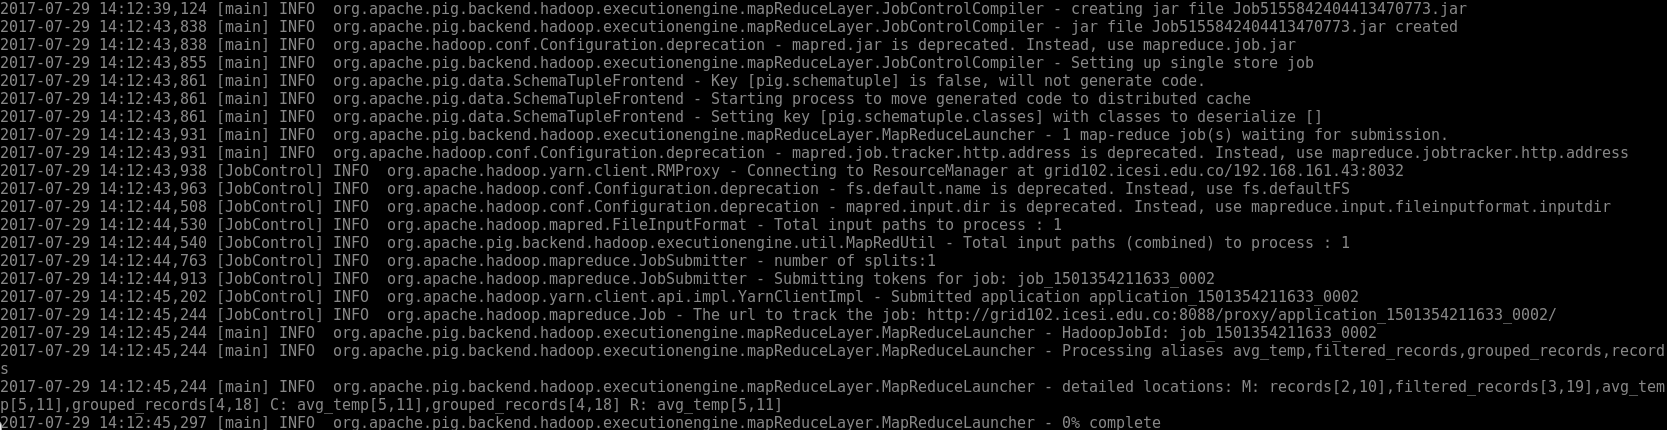
\includegraphics[width=\textwidth, height=2.0in]{fig/05/04}
  \caption{Monitoreo de la ejecución del programa \textit{AverageTemperature} en Pig por medio de la consola Grunt desde donde se ejecutó.}
\end{figure}

\begin{figure}[H]
  \centering
      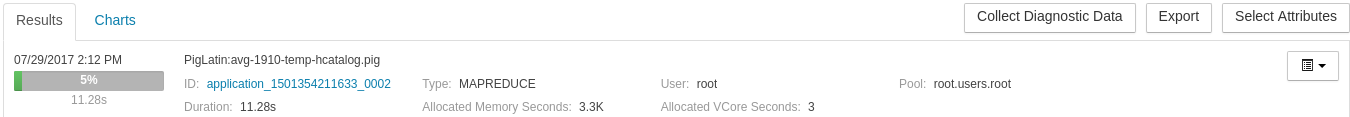
\includegraphics[width=\textwidth, height=0.8in]{fig/05/05}
  \caption{Monitoreo de la ejecución del programa \textit{AverageTemperature} en Pig por medio de la interfaz de YARN.}
\end{figure}

\begin{figure}[H]
  \centering
      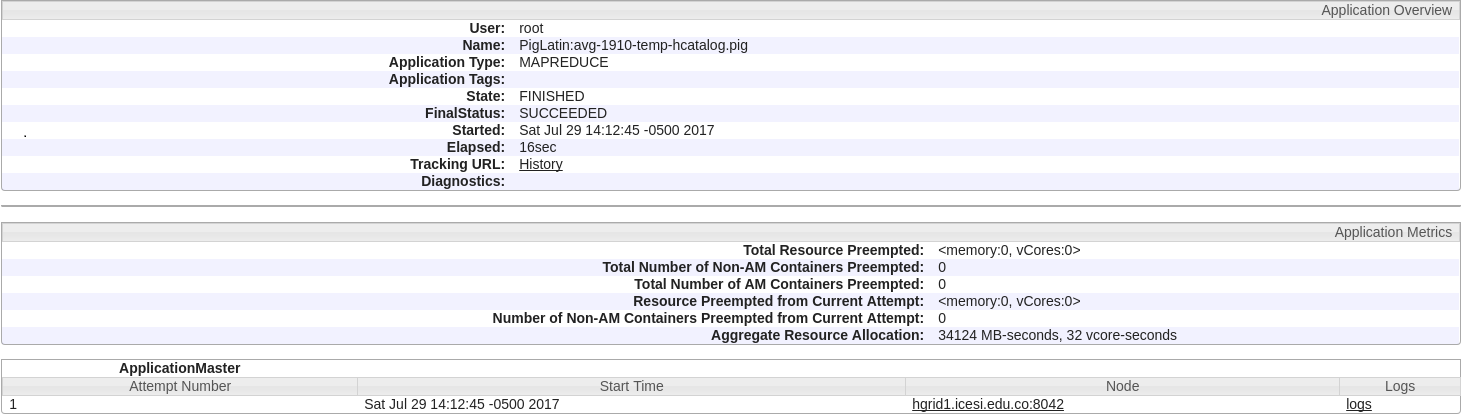
\includegraphics[width=\textwidth, height=2.7in]{fig/05/06}
  \caption{Ejecución finalizada, vista desde el Job History Server.}
\end{figure}

\section{Oozie}
En esta sección se presentan las ejecuciones realizadas con Apache Oozie para el objetivo específico 4 del presente proyecto.

\subsection{Problemas tratados}

\subsubsection{Problema 1:} Determinar la temperatura máxima promedio registrada en cada día del año para cada estación metereológica, teniendo como base los datos consignados en el dataset del NCDC. Ejemplo: 029070-99999 0101 -68.

\subsubsection{Problema 2:} Mejorar los tiempos de ejecución del problema 1.

\subsection{Estrategia general para el Problema 1}

La estrategia para abordar el primer problema consiste en realizar dos pasos \textit{stages} 

\begin{enumerate}

\item Calcular la temperatura máxima diaria para cada llave estación-fecha. Ejemplo: 29070-99999 19020101 -94.

\item Calcular el promedio de las temperaturas diarias para cada llave estación-mes. Ejemplo: 029070-99999 0101 -68.

\end{enumerate}

\subsection{Estrategia problema 2: Apache Oozie, Hive y Pig}

A continuación se detallan los pasos necesarios para resolver el problema 2, usando Oozie, Hive y Pig. \\

\subsubsection{Definición de tabla} Para facilitar el cambio del primer \textit{stage} por un script de Hive (inicialmente está escrito en Pig), se decidió darle un nuevo formato a los datos del NCDC. A continuación se presenta el script utilizado para crear una nueva tabla de Hive con el nuevo formato de los datos.

\begin{lstlisting}[linewidth=\columnwidth,breaklines=true]
ADD jar /usr/lib/&hiv&e/lib/&hive&-contrib-1.1.0-cdh5.10.1.jar;

CREATE TABLE weather_managed_lf
AS SELECT
CAST(CONCAT(usaf,'-',wban) AS STRING),  CAST(CONCAT(observation_date_year,observation_date_month,observation_date_day) AS INT),
        CAST(air_temperature AS INT),
        CAST(at_quality_code AS INT)
    FROM weather_external;
\end{lstlisting}

\subsubsection{Definición de los parámetros del \textit{workflow}} Así como Pig y Hive, Oozie permite la definición de parámetros para la ejecución de \textit{workflows}. A continuación se presenta el archivo \textit{workflow.properties}, el cual contiene los parámetros necesarios para la correcta ejecución de la aplicación de Oozie. 

\begin{lstlisting}[linewidth=\columnwidth,breaklines=true]
nameNode=hdfs:&//grid101.icesi.edu.co:8020&
resourceManager=grid102.icesi.edu.co:8032
&oozie&.wf.application.path=${nameNode}/user/${user.name}/mean-max-temp-workflow-&hive&-&pig&
# Output for stage 1.
outS1Dir=${nameNode}/user/${user.name}/&hive&-&pig&-s1-out
# Input &for& stage 2.
inS2Dir=${outS1Dir}
# Output &for& stage 2.
outS2Dir=${nameNode}/user/${user.name}/&hive&-&pig&-s2-out
&oozie&.use.system.libpath=true
&oozie&.libpath=${nameNode}/user/&oozie&/share/lib
\end{lstlisting}

\subsubsection{Definición del primer stage} A continuación se presenta el archivo \textit{s1Hive.sql}, el cual contiene la definición del primer \textit{stage} del \textit{workflow} en cuestión.

\begin{lstlisting}[linewidth=\columnwidth,breaklines=true]
ADD jar /usr/lib/&hive&/lib/&hive&-contrib-1.1.0-cdh5.10.1.jar;
INSERT OVERWRITE DIRECTORY '${outS1}'
ROW FORMAT DELIMITED
FIELDS TERMINATED BY '	' 	
SELECT `_c0`, `_c1`, MAX(air_temperature) FROM weather_managed_lf 
WHERE at_quality_code IN (0,1,4,5,9) AND air_temperature <> 9999
GROUP BY `_c0`,`_c1`;
\end{lstlisting}

\subsubsection{Definición del segundo stage} A continuación se presenta el archivo \textit{s2.pig}, el cual contiene la definición del segundo \textit{stage} del \textit{workflow} en cuestión.

\begin{lstlisting}[linewidth=\columnwidth,breaklines=true]
records = LOAD '$inS2' AS (station:chararray,date:chararray,temperature:int);
formated_records = FOREACH records GENERATE station, SUBSTRING(date, 4, 8), temperature;
grouped_records = GROUP formated_records BY ($0,$1);
mean_station_day_month = FOREACH grouped_records GENERATE FLATTEN(group),AVG(formated_records.temperature);
STORE  mean_station_day_month INTO '$outS2';
\end{lstlisting}

\subsubsection{Definición del workflow} A continuación se presenta el archivo \textit{workflow.xml}, el cual define el \textit{workflow} que será ejecutado con Oozie.

\lstinputlisting[language=xml]{workflow2.xml}

\subsubsection{Ejecución del \textit{workflow}} A continuación se presentan los pasos necesarios para ejecutar el \textit{workflow} de Oozie.

\begin{lstlisting}[linewidth=\columnwidth,breaklines=true]
#Remove &oozie& app.
hadoop fs -rm -r mean-max-temp-workflow-&hive&-&pig&

#Copy &oozie& app.
hadoop fs -put /home/sas6/Oozie-Pig-HCatalog-Demos/src/&oozie&/&hive&-&pig&/mean-max-temp-workflow-&hive&-&pig& mean-max-temp-workflow-&hive&-&pig&

#Oozie server
export OOZIE_URL="http://grid102.icesi.edu.co:11000/oozie"

#Run job
oozie job -config /home/sas6/Oozie-Pig-HCatalog-Demos/src/&oozie&/&hive&-&pig&/mean-max-temp-workflow-&hive&-&pig&/workflow.properties -run
\end{lstlisting}



\subsection{Seguimiento a la ejecución del workflow}

El monitoreo de la ejecución del workflow podrá realizarse a través del servidor de Oozie.

\begin{figure}[H]
  \centering
      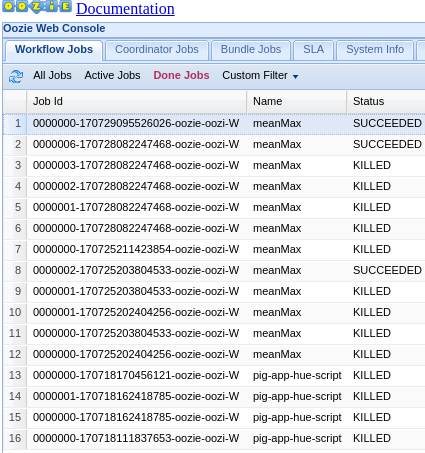
\includegraphics[width=\textwidth, height=5.0in]{fig/06/01}
  \caption{Lista de \textit{jobs} de Oozie ejecutados.}
\end{figure}

\begin{figure}[H]
  \centering
      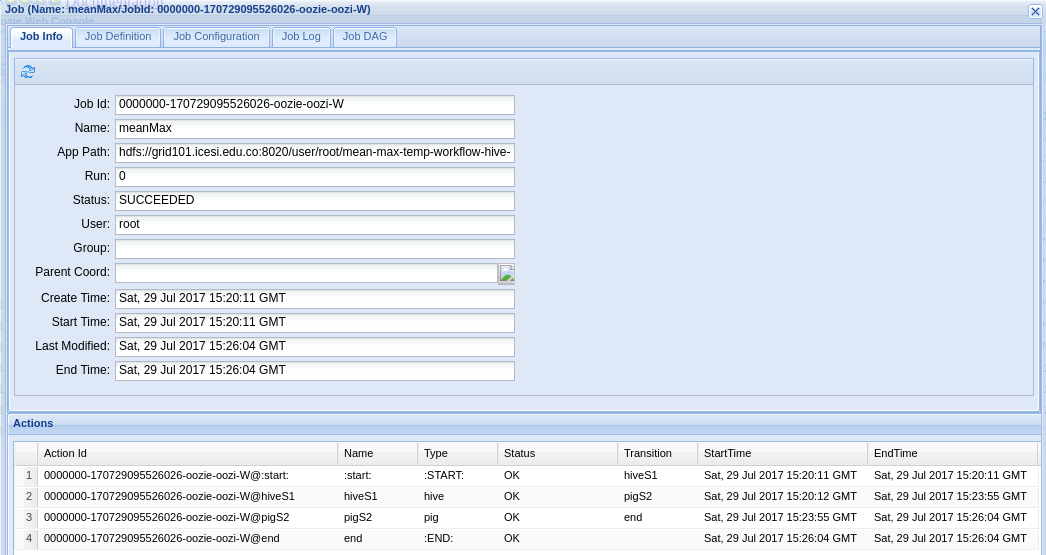
\includegraphics[width=\textwidth, height=5.0in]{fig/06/02}
  \caption{Detalle del \textit{job} de Oozie ejecutado.}
\end{figure}

\begin{figure}[H]
  \centering
      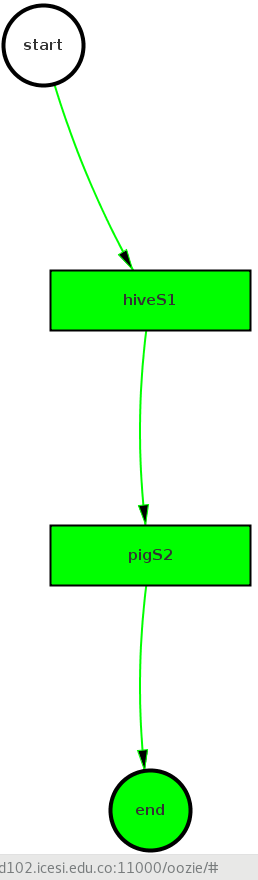
\includegraphics[width=3.0in, height=6.0in]{fig/06/03}
  \caption{Ejecución finalizada, vista desde el grafo acíclico dirigido generado desde la UI del servidor de Oozie.}
\end{figure}

\section{Results}
En esta sección se presentan los resultados obtenidos a partir de las distintas ejecuciones realizadas. \\

\subsection{Resultados objetivo específico 1: MapReduce vs Hive (\textit{external tables}) vs Pig}

A continuación se ilustran los distintos tiempos de ejecución obtenidos a partir de las pruebas realizadas con el programa \textit{MaxTemperature} en las versiones MapReduce-Java, Pig, y Hive para el total y el 10\% de los datos del NCDC. La figura \ref{07_01_01} compara los tiempos de ejecución del programa \textit{MaxTemperature} en la versión MapReduce-Java con el total y el 10\% de los datos. La figura \ref{07_01_02} compara los tiempos de ejecución del programa \textit{MaxTemperature} en la versión Pig con el total y el 10\% de los datos. La figura \ref{07_01_03} compara los tiempos de ejecución del programa \textit{MaxTemperature} en versión Hive en su forma nativa (Hive server) y desde Hue (\textit{managed tables}) con el total de los datos. La figura \ref{07_01_04} compara los tiempos de ejecución del programa \textit{MaxTemperature} en las versiones MapReduce-Java, Hive (\textit{external tables}), y Pig con el total de los datos.

\begin{figure}[H]
  \centering
      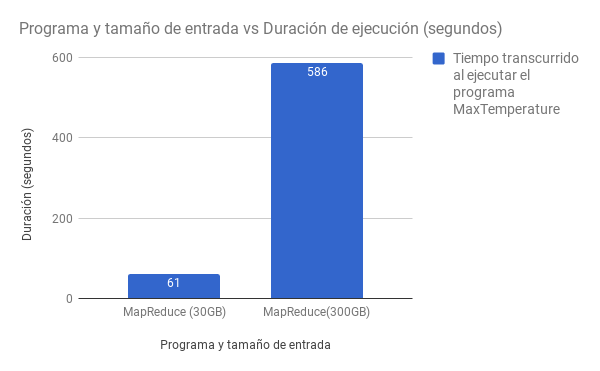
\includegraphics[width=\textwidth, height=3.0in]{fig/07/01_01}
  \caption{Comparación de MapReduce-Java con el total y el 10\% de los datos.}
  \label{07_01_01}
\end{figure}

\begin{figure}[H]
  \centering
      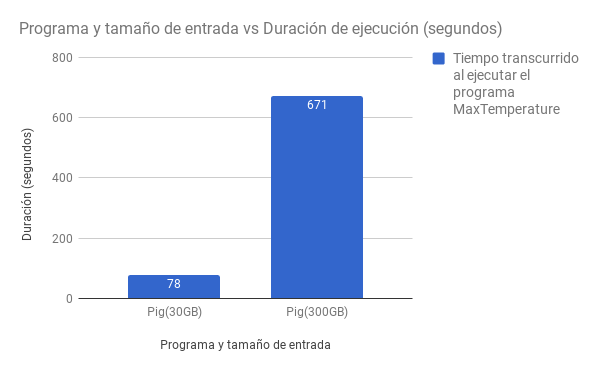
\includegraphics[width=\textwidth, height=3.0in]{fig/07/01_02}
  \caption{Comparación de Pig con el total y el 10\% de los datos.}
  \label{07_01_02}
\end{figure}

\begin{figure}[H]
  \centering
      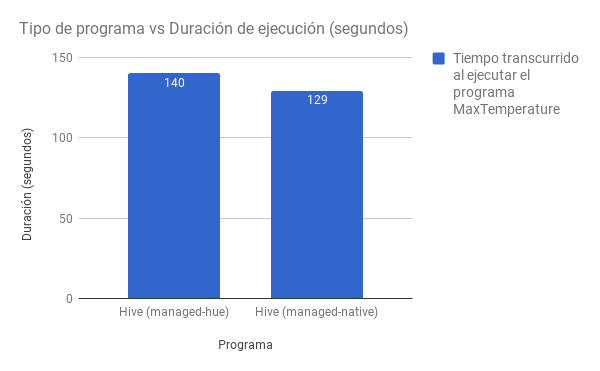
\includegraphics[width=\textwidth, height=3.0in]{fig/07/01_03}
  \caption{Comparación de ejecución en Hive de forma nativa y desde Hue con el total de los datos.}
  \label{07_01_03}
\end{figure}

\begin{figure}[H]
  \centering
      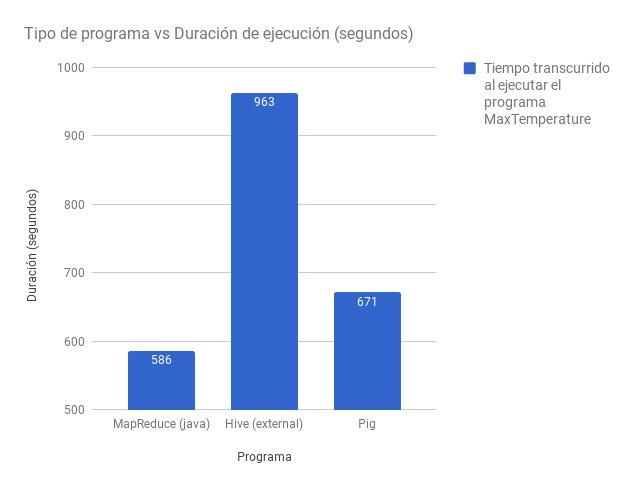
\includegraphics[width=\textwidth, height=3.5in]{fig/07/01_04}
  \caption{Comparación de ejecución del programa \textit{MaxTemperature} desde MapReduce, Hive (\textit{external table}), y Pig con el total de los datos.}
  \label{07_01_04}
\end{figure}

\subsection{Resultados objetivo específico 2: Escalabilidad en Pig}

A continuación se ilustran los distintos tiempos de ejecución obtenidos a partir de las pruebas realizadas con el programa \textit{AverageTemperatureCount} para medir la escabilidad de Pig. Para esto, dos distintos enfoques fueron usados: el primero consistía en deshabilitar, mediante la interfaz gráfica de YARN, NodeManagers y trabajar con el total de DataNodes (10 en nuestro caso); el segundo consistía en agregar nuevos nodos al cluster y ejecutar los scripts cada vez que esto sucedía, lo que significaba que las instancias de NodeManagers activas eran igual a los nodos en los que se encontraban replicados los datos. La figura \ref{07_02_01} muestra los resultados del primer enfoque, mientras que la figura \ref{07_02_02} muestra los del segundo.

\begin{figure}[H]
  \centering
      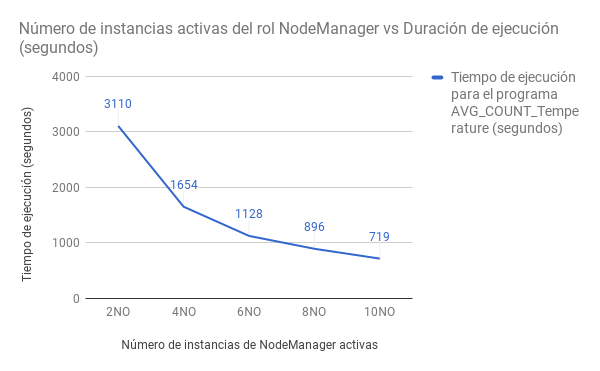
\includegraphics[width=\textwidth, height=3.0in]{fig/07/02_01}
  \caption{Escalabilidad de Pig en términos del procesamiento de datos (Pig/YARN).}
  \label{07_02_01}
\end{figure}

\begin{figure}[H]
  \centering
      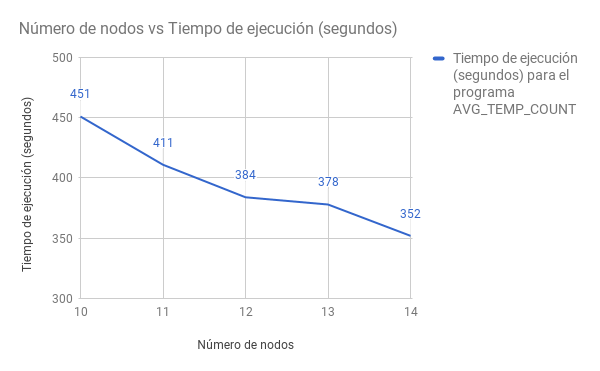
\includegraphics[width=\textwidth, height=3.0in]{fig/07/02_02}
  \caption{Escalabilidad de Pig (Pig/HDFS/YARN).}
  \label{07_02_02}
\end{figure}

Para analizar los resultados evidenciados en las gráficas anteriores, se transformaron los tiempos de ejecución (eje vertical) a una escala logarítmica y se uso la función \textit{lm} del lenguaje de programación R para comprobar si en efecto la escalabilidad era logarítmica. A continuación se presentan los resultados arrojados. \\

\subsubsection{Análisis de la escalabilidad de Pig siguiendo el enfoque 1}

\begin{itemize}

\item \textbf{Función de transformación:} $log(y)$
\item \textbf{p-value:} 0.002416

\end{itemize}

\subsubsection{Análisis de la escalabilidad de Pig siguiendo el enfoque 2}

\begin{itemize}

\item \textbf{Función de transformación:} $log(y)$
\item \textbf{p-value:} 0.004018

\end{itemize}

\subsection{Resultados objetivo específico 3: Extensibilidad de Pig con HCatalog:}

A continuación se ilustran los distintos tiempos de ejecución y tamaños de lectura de datos desde HDFS obtenidos a partir de las pruebas realizadas con el programa \textit{AverageTemperature} para medir la extensibilidad de Pig con HCatalog y su influencia en los tiempos de ejecución. La figura \ref{07_03_01} muestra la comparación en los tiempos de ejecución para el programa \textit{AverageTemperature-1950} de Pig con HCatalog (con una tabla no particionada), Pig con HCatalog (con una tabla particionada), y de Pig sin HCatalog. La figura \ref{07_03_02} muestra la comparación de la lectura de datos desde HDFS para el programa \textit{AverageTemperature-1950} de Pig con HCatalog (con una tabla no particionada), Pig con HCatalog (con una tabla particionada), y de Pig sin HCatalog. La figura \ref{07_03_03} muestra la comparación en los tiempos de ejecución para el programa \textit{AverageTemperature-1910} de Pig con HCatalog (con una tabla no particionada), Pig con HCatalog (con una tabla particionada), y de Pig sin HCatalog. La figura \ref{07_03_04} muestra la comparación de la lectura de datos desde HDFS para el programa \textit{AverageTemperature-1910} de Pig con HCatalog (con una tabla no particionada), Pig con HCatalog (con una tabla particionada), y de Pig sin HCatalog.


\begin{figure}[H]
  \centering
      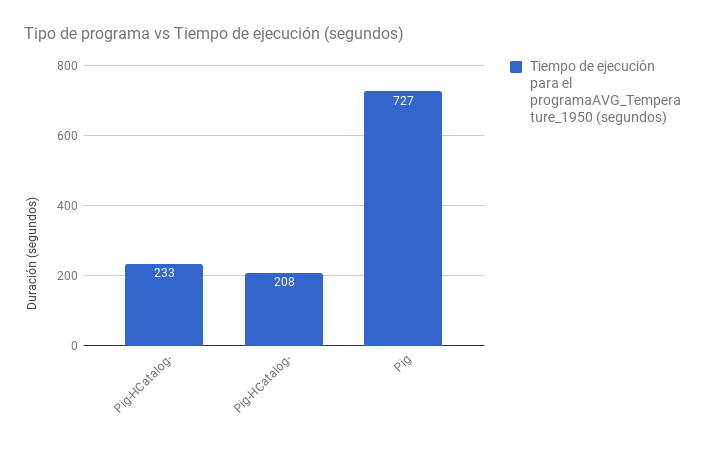
\includegraphics[width=\textwidth, height=4.0in]{fig/07/03_01}
  \caption{Tiempos de ejecución obtenidos para el programa \textit{AverageTemperature-1950}.}
  \label{07_03_01}
\end{figure}

\begin{figure}[H]
  \centering
      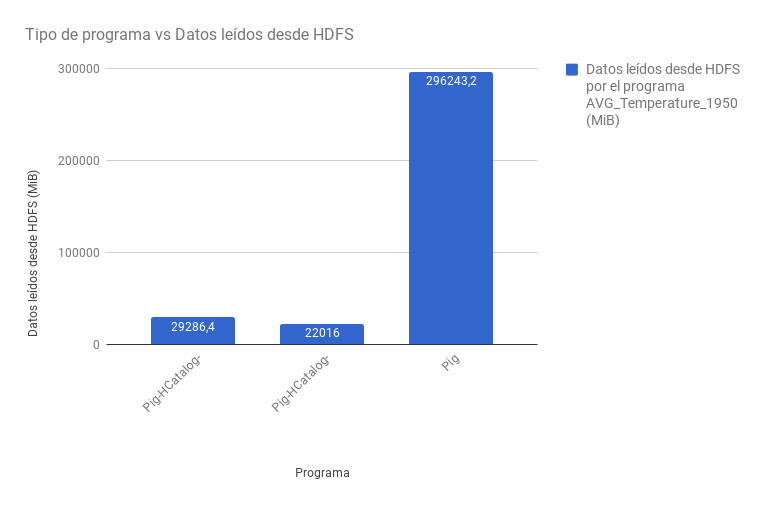
\includegraphics[width=\textwidth, height=4.0in]{fig/07/03_02}
  \caption{Lectura de datos desde HDFS para el programa \textit{AverageTemperature-1950}.}
  \label{07_03_02}
\end{figure}

\begin{figure}[H]
  \centering
      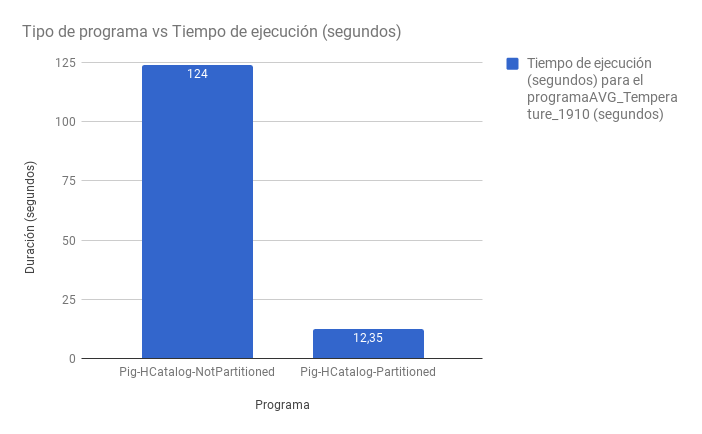
\includegraphics[width=\textwidth, height=4.0in]{fig/07/03_03}
  \caption{Tiempos de ejecución obtenidos para el programa \textit{AverageTemperature-1910}.}
  \label{07_03_03}
\end{figure}

\begin{figure}[H]
  \centering
      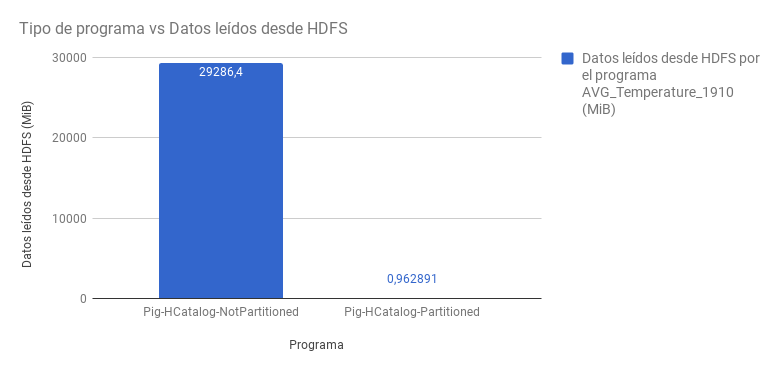
\includegraphics[width=\textwidth, height=4.0in]{fig/07/03_04}
  \caption{Lectura de datos desde HDFS para el programa \textit{AverageTemperature-1910}.}
  \label{07_03_04}
\end{figure}

\subsection{Resultados objetivo específico 4: Reusabilidad y mantebilidad en Oozie}

La reusabilidad y mantenibilidad de los \textit{workflows} de Oozie se pudo comprobar al lograr intercambiar fácilmente el primer \textit{stage} del mismo.  La figura \ref{07_04_01} ilustra los tiempos de ejecución obtenidos a partir de las pruebas realizadas con las definiciones del \textit{workflow} en sus versiones: Pig-Pig y Hive-Pig.

\begin{figure}[H]
  \centering
      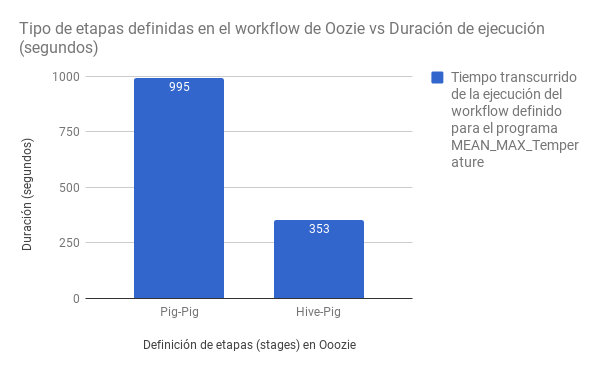
\includegraphics[width=\textwidth, height=4.0in]{fig/07/04_01}
  \caption{Comparación del \textit{workflow} de Oozie con la combinación Pig-Pig y Hive-Pig.}
  \label{07_04_01}
\end{figure}

\section{Conclusions}
Las pruebas realizadas en este proyecto indican en un principio que: \\

\begin{itemize}

\item Respecto al objetivo específico 1, en términos de tiempos de ejecución, Hive (con \textit{external tables}) ejecuta las actividades en un tiempo significativamente mayor que MapReduce y Pig.  Además, como era de esperarse, Pig realiza procesamientos en los datos en un tiempo mayor a MapReduce en su versión Java.

\item Respecto al objetivo específico 1, Hue no parece adicionar un \textit{overhead} importante sobre las consultas realizadas en Hive, sin embargo, aunque leve, si hay un costo de realizar la planeación de las ejecuciones con Oozie cuando se ejecutan las consultas desde Hue.

\item Respecto al objetivo específico 2, aparentemente, la escalabilidad de Pig no es del todo lineal sino logarítmica.

\item Respecto al objetivo específico 3, Pig es un framework extensible que puede aprovechar las ventajas de Hive (\textit{metastore} y tablas particionadas) a través de HCatalog. Sin embargo, no parece haber compatibilidad con tablas externas de Hive.

\item Respecto al objetivo específico 4, la reusabilidad y mantenibilidad de los workflows de Oozie se pudo comprobar a través del presente proyecto, pues fue relativamente sencillo actualizar el \textit{workflow} inicial para dar soporte a las nuevas necesidades (mejoras en el rendimiento a partir de las ventajas de Hive).

\end{itemize}


Es importante aclarar que las conclusiones listadas previamente son el reflejo de las ejecuciones de las distintas tecnologías del ecosistema de Hadoop que fueron tratadas en este proyecto. No deben ser consideradas como conclusiones definitivas, pues se necesitaría un mayor número de pruebas y estudio más completo de las distintas herramientas utilizadas para los fines de este proyecto.

\section{Future work}
A continuación se enuncian aquellas actividades que, por una u otra razón, no fueron tratadas en el contexto del presente proyecto, sin embargo, podrían hacer parte de futuras discusiones. \\

\begin{enumerate}

\item Comparar el rendimiento de Apache Oozie frente a otras alternativas como Apache Falcon o Apache NiFi.

\item Explorar cómo se podrían aprovechar las tablas de Hive con buckets desde Pig, mediante HCatalog.

\end{enumerate}
% references section

% can use a bibliography generated by BibTeX as a .bbl file
% BibTeX documentation can be easily obtained at:
% http://www.ctan.org/tex-archive/biblio/bibtex/contrib/doc/
% The IEEEtran BibTeX style support page is at:
% http://www.michaelshell.org/tex/ieeetran/bibtex/
%\bibliographystyle{IEEEtran}
% argument is your BibTeX string definitions and bibliography database(s)
%\bibliography{IEEEabrv,../bib/paper}
%
% <OR> manually copy in the resultant .bbl file
% set second argument of \begin to the number of references
% (used to reserve space for the reference number labels box)
\begin{thebibliography}{1}

\bibitem{IEEEhowto:kopka}
H.~Kopka and P.~W. Daly, \emph{A Guide to \LaTeX}, 3rd~ed.\hskip 1em plus
  0.5em minus 0.4em\relax Harlow, England: Addison-Wesley, 1999.

\end{thebibliography}

% biography section
% 
% If you have an EPS/PDF photo (graphicx package needed) extra braces are
% needed around the contents of the optional argument to biography to prevent
% the LaTeX parser from getting confused when it sees the complicated
% \includegraphics command within an optional argument. (You could create
% your own custom macro containing the \includegraphics command to make things
% simpler here.)
%\begin{biography}[{\includegraphics[width=1in,height=1.25in,clip,keepaspectratio]{mshell}}]{Michael Shell}
% or if you just want to reserve a space for a photo:

%\begin{IEEEbiography}[{\includegraphics[width=1in,height=1.25in,clip,keepaspectratio]{picture}}]{John Doe}
%\blindtext
%\end{IEEEbiography}

% You can push biographies down or up by placing
% a \vfill before or after them. The appropriate
% use of \vfill depends on what kind of text is
% on the last page and whether or not the columns
% are being equalized.

%\vfill

% Can be used to pull up biographies so that the bottom of the last one
% is flush with the other column.
%\enlargethispage{-5in}




% that's all folks
\end{document}


